\documentclass[10pt,a4paper]{article}
\usepackage[margin=1.7cm]{geometry}
\usepackage{amsmath,amssymb,graphicx,xcolor,enumitem,booktabs}
\usepackage[hidelinks]{hyperref}
\graphicspath{{../paper/prl/figs/}{../tilt_report/figs/}}
\DeclareGraphicsExtensions{.pdf,.png}
\setlist{itemsep=1pt,topsep=2pt,leftmargin=1.2em}
\newcommand{\half}{\tfrac12}\newcommand{\la}{\ell_a}\newcommand{\kT}{k_BT}
\pagestyle{empty}
\begin{document}
\noindent{\Large\textbf{Overcharged active nematic cavities: briefing}}\hfill 21 October 2026\\[2pt]
B.~Loewe and T.~N.~Shendruk (prepared with Claude). Details: theory report (33 pp), tilt report (11 pp), PRL drafts v1/v2, SI.

\section*{1. The story (PRL v2 framing: geometry over topology)}
\begin{itemize}
\item \textbf{Observation.} A cavity whose anchoring winds $k$ times holds charge $k$. Passive: all $2k$ $+\half$ at the wall. Active circles ($0.8\lesssim R/\la\lesssim2.2$, $k=2$--10, 10 seeds): exactly $2k-2$ at the wall and a net $+1$ in the bulk.
\item \textbf{Geometry sets the count.} The anchoring turns by $(k-1)\phi$ relative to the normal: $2k-2$ homeotropic sites, and each wall defect's tilt is locked to its position (resultant 0.99). Only a ring of $2|k-1|$ can tilt as a whole.
\item \textbf{The coherent flow lets geometry act.} The active vortex imposes a common tilt; the $2k$ ring cannot follow and ejects two defects (forcing a common tilt on it costs 375--475\,$\kT$ at $k=6$, ejection 180--200). A \emph{passive} cavity under an imposed vortex does the same; so does a continuum active nematic.
\item \textbf{Elongation removes the flow.} Above aspect $\approx1.3$ the vortex breaks, wall defects untilt, their jets turn inward and they escape; the bulk charge follows a wall law (fixed charge per wall length). Higher $\lambda$ does not rescue it.
\item \textbf{Controls.} Negative winding ($-\half$ walls, no jets): same vortex loss, no leak ($0.05$ vs $2.0$ defects lost, escapes $\approx30\times$ rarer). Seeded $-k$ starts: no creation barrier, the count is set by retention. Pressure-driven channels: a strong coherent shear re-screens flat walls completely (12 of 12), weak spontaneous flow does not. Robust at $\zeta=0.06$, 0.08.
\item \textbf{Tilt angle} (supporting): $\arccos(1/\lambda)$ in sparse layers, within $3^\circ$ for $\lambda=2$--6.
\end{itemize}
\begin{center}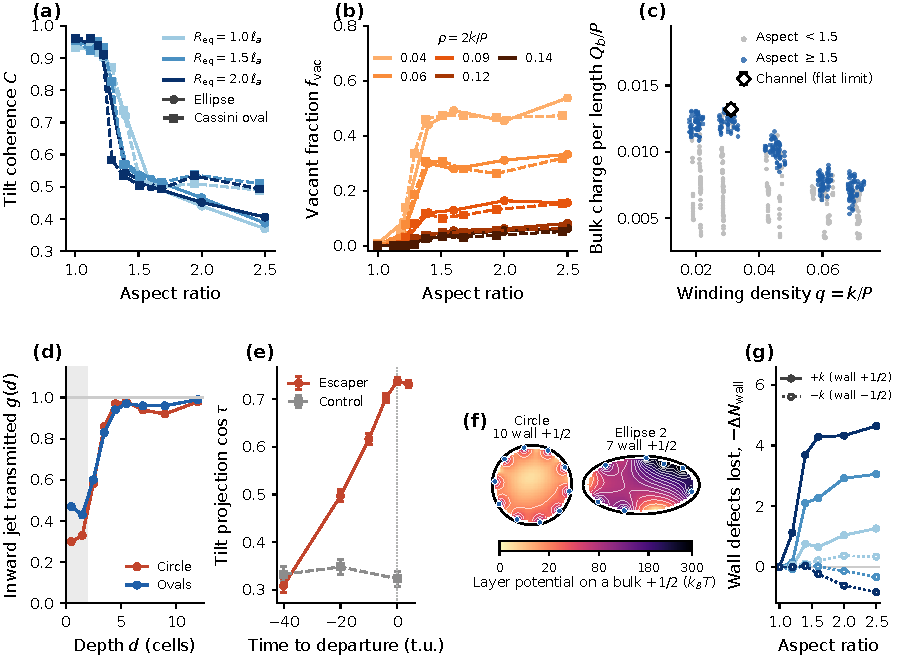
\includegraphics[width=0.98\textwidth]{fig4_shapes}\\[-2pt]
{\small PRL Fig.~4: elongation breaks coherence and empties the layer (a, b); wall law (c); jet blocking and untilting (d, e); shielding (f); mirror control (g).}\end{center}

\section*{2. Open: crowded layers tilt less}
\begin{itemize}
\item \textbf{Measured.} Coherent-layer tilt $64.6^\circ\to44^\circ$ as the wall-defect spacing falls from $>20$ to 7 cells; same in passive layers under an imposed vortex and in every shape; ordered by core depth over alignment length ($d\sqrt{s}$), which predicts an independent shear scan; drop $15^\circ\to<1^\circ$ from $\lambda=2$ to 6. Not noise (MPCD at twice the density: same crowded tilt).
\item \textbf{Pinning.} \emph{Site} pinning is settled ($K_1\neq K_3$ pins the commensurate ring, 80--110\,$\kT$). What is open is the \emph{restoring torque against the flow}: the static registry stiffness weakens with crowding (19 to 0.2--0.4\,$\kT$/rad$^2$), and with $K_1>K_3$ a flat wall prefers the opposite sign.
\item \textbf{Continuum.} A drop below $60^\circ$ appears only when the elastic pull points to the untilted registry ($K_1/K_3=0.55$), or when the activity is strong: $8^\circ$ at $\zeta=3$ (laminar, full spiral), rising to $10.7^\circ$ at $\zeta=8$ (turbulent bulk) -- about half to three-quarters of MPCD's $14^\circ$ at the same spacings. Turbulence vs stronger wall shear: control running today.
\end{itemize}
\begin{center}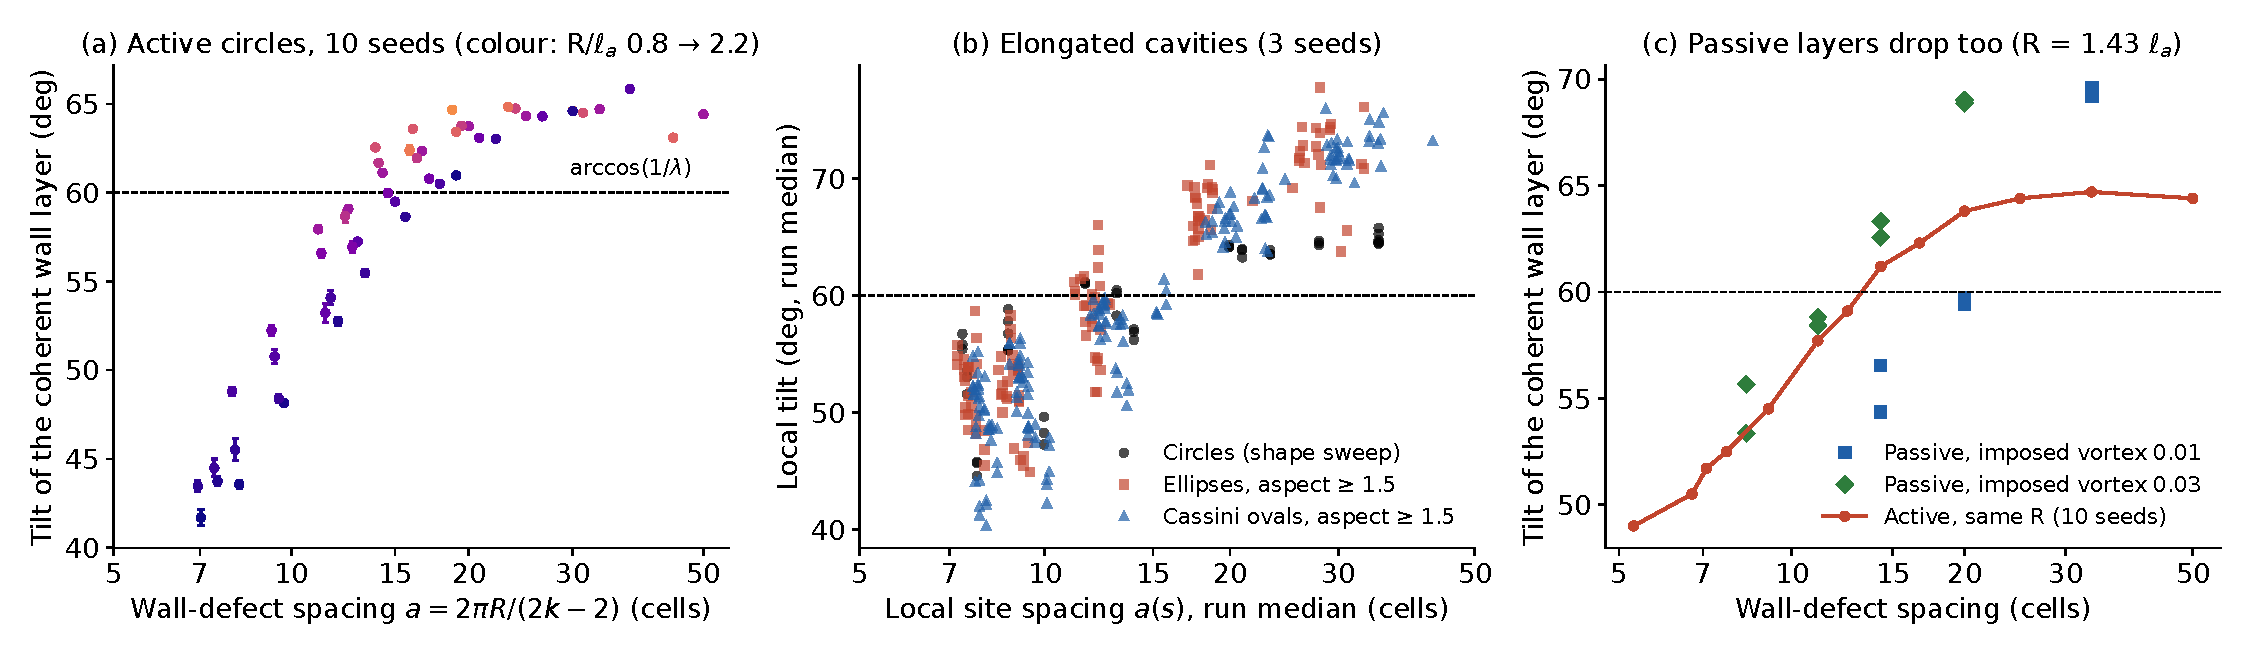
\includegraphics[width=0.98\textwidth]{../tilt_report/figs/fig1_observation}\\[-2pt]
{\small Tilt report Fig.~1: (a) active circles, 10 seeds; (b) elongated cavities (local); (c) passive layers drop too.}\end{center}

\section*{3. Questions for Tyler}
\begin{enumerate}
\item \textbf{Crowded layers:} where could a restoring torque towards the untilted registry come from in MPCD? Ideas for a minimal model (the disordered bulk next to an ordered ring?).
\item \textbf{Framing and title:} v1 ``Flow alignment sets the topological charge\ldots'' vs v2 ``Geometry, not topology, places the charge\ldots''. Or a combination.
\item \textbf{PRL vs SI:} which of shielding/vacancy maps, mirror control, continuum and channels-as-flat-limit go in the main text (PRL $\approx3750$ words, 4 figures; currently $\approx3200$).
\item \textbf{Is the crowding drop a paper result or a caveat?} We state $\arccos(1/\lambda)$ as the sparse-layer limit and report the drop in the SI.
\item \textbf{Experiments:} which systems (microtubule--kinesin in patterned wells, cell monolayers) and references to cite.
\item \textbf{Channels} (separate paper): $J\propto1/W$ topological current, narrow-channel screening crossover $W^*\propto1/m$, pressure-driven re-screening, ``surfing'' $+\half$ on bend jets. Scope and timing?
\end{enumerate}
\end{document}
